\chapter{[Właściwy dla kierunku - np.Specyfikacja wewnętrzna]}
Jeśli to Specyfikacja wewnętrzna:
\begin{itemize}
\item przedstawienie idei
\item architektura systemu
\item opis struktur danych (i organizacji baz danych)
\item komponenty, moduły, biblioteki, przegląd ważniejszych klas (jeśli występują)
\item przegląd ważniejszych algorytmów (jeśli występują)
\item szczegóły implementacji wybranych fragmentów, zastosowane wzorce projektowe
\item diagramy UML
\end{itemize}


\begin{itemize}
\item wymagania funkcjonalne i niefunkcjonalne
\item przypadki użycia (diagramy UML) - dla prac, w których mają zastosowanie
\item opis narzędzi, metod eksperymentalnych, metod modelowania itp.
\item metodyka pracy nad projektowaniem i implementacją - dla prac, w których ma to zastosowanie
\end{itemize}

\section{Klasa OpenLeap}

\subsection{Relacja klas - kompozycja}
\quad Klasa OpenLeap korzysta z różnych bibliotek oraz klas. Natomiast nie dziedziczy ona żadnej klasy. Zostały jedynie wykorzystane wybrane metody tworzonych obiektów wewnątrz klasy. 

\begin{figure}[H]
    \begin{center}
        \includegraphics[width=10cm]{example-image-a}
        \caption{Relacja klas} 
    \end{center}
\end{figure}

\quad OpenLeap wykorzstuje metody klasy \textbf{mediapipe.solutions.hands.Hands} oraz \textbf{cv2.VideoCapture}. Pierwsza klasa pozwala na stworzenie obiektu, któreg zadaniem jest rozpoznawanie dłoni na podstawie podawanego obrazu. Druga klasa tworzy obiekt, który pozwala na pobranie obrazu z kamery, określenie jego wielkości oraz sprawdzenia czy kamery jest aktualnie dostępna. 

\subsection{Budowa klasy}

\quad 

\begin{figure}[H]
    \begin{center}
        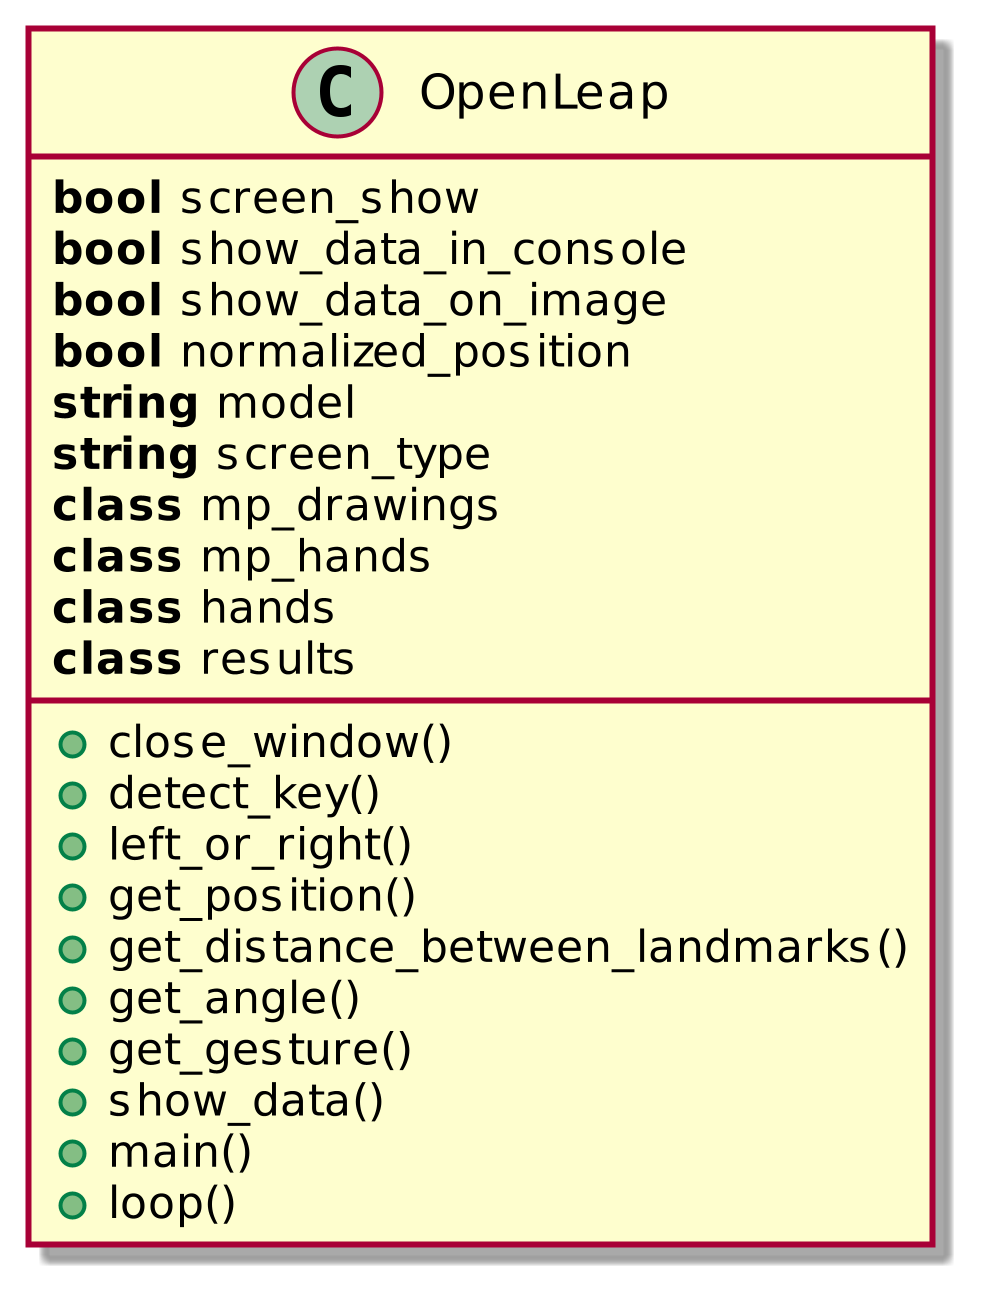
\includegraphics[width=10cm]{../images/class.png}
        \caption{Schemat klasy OpenLeap} 
    \end{center}
\end{figure}

\subsection{Atrybuty klasy}

\quad Część atrybutów klasy została opisana w podrozdziale \textbf{\nameref{parametry}}, są to te elementy, które mogą zostać zdefiniowane przez użytkownika. Druga część atrybutów jest generowana automatycznie. 

\begin{itemize}
    \item \textbf{mp\_drawings} - obiekt pobierany z bilbioteki \textbf{MediaPipe} pozwalająca na rysowanie obrysu dłoni w oknie generowanym przez OpenCV.
    \item \textbf{mp\_hands} - obiekt przechowujący informacje, na przykład o indeksach opisujących poszczególne elementy charakterystyczne dłoni. 
    \item \textbf{hands} - model biblioteki MediaPipe rozpoznający dłonie. Inicjalizacja tego obiektu wymaga podnania dwóch parametrów. 
    \begin{itemize}
        \item \textbf{min\_detection\_confidence} - minimalna wartość szacunkowa, dla której model określa czy została wykryta dłoń.
        \item \textbf{min\_tracking\_confidence} - minilana wartość szacunkowa, pozwalająca określić dokładność śledzenia dłoni. 
    \end{itemize}
    \item \textbf{results} - obiekt przechowujący informacje o rozpoznanych dłoniach i ich elementach. 
\end{itemize}

\subsection{Metody klasy}

\begin{enumerate}
    \item \textbf{close\_window()} - zamknięcie wszytkich okien biblioteki OpenCV.
    \item \textbf{detect\_key()} - wykrycie kliknięcia wybranego przycisku podanego w argumencie.
    \item \textbf{left\_or\_right()} - metoda rozpoznająca lewą oraz prawą dłoń. Metoda za arugmenty przyjmuje:
    \begin{itemize}
        \item \textbf{index} - indeks badanej dłoni. 
        \item \textbf{mode} - metoda określania typu dłoni. 
        \begin{itemize}
            \item \textbf{AI} - wykorzystuje gotowy model MediaPipe. Niestety ten może nie zawsze działać poprawnie. 
            \item \textbf{position} - drugą metodą jest bazowanie na pozycji dłoni, dłoń po prawej stronie względem drugiej dłoni jest dłonią prawą i odwrotnie. Jeśli na ekranie widoczna jest jedna dłoń, wtedy funkcja jest wywoływana ponownie z metodą 'AI'.
        \end{itemize}
        \item \textbf{hand} - obiekt przechowujący współrzędne elementów charakterystycznych danej dłoni. 
    \end{itemize}
    \item \textbf{get\_position()} - Funkcja zwraca pozycję elementu danej dłoni. 
    \begin{itemize}
        \item \textbf{index} - indeks badanej dłoni. 
        \item \textbf{landmark\_idx} - indeks elementu charakterystycznego, którego pozycję ma zwrócić funkcja. 
        \item \textbf{normalized} - parametr określający czy zwrócone współrzędne mają zostać znoramalizowane czy nie. 
    \end{itemize}
    \item \textbf{get\_distance\_between\_landmarks()} - Metoda obliczająca odległość między dwoma wybranymi elementami charakterystycznymi.
    \begin{itemize}
        \item \textbf{index} - indeks dłoni, na której znajdują się mierzone elementy. 
        \item \textbf{landmark\_1} - indeks pierwszego elementu dłoni. 
        \item \textbf{landmark\_2} - indeks drugiego elementu dłoni. 
        \item \textbf{normalized} - parametr określający czy odległość ma zostać znomralizowana. 
    \end{itemize}
    \item \textbf{get\_angle()} - metod zwracająca kąt obrotu wybranego elementu charakterystycznego dłoni względem nadgarstka. 
    \begin{itemize}
        \item \textbf{index} - indeks wybranej dłoni. 
        \item \textbf{landmark\_idx} - indeks elementu względem, którego obliczany jest kąt. 
        \item \textbf{mode}
        \begin{itemize}
            \item \textbf{half} - zwraca kąt półpełny
            \item \textbf{full} - zwraca kąt pełny
        \end{itemize}
        \item \textbf{unit}
        \begin{itemize}
            \item \textbf{radians} - jednostka kąta w radianach
            \item \textbf{degrees} - jednostka kąta w stopniach
        \end{itemize}
    \end{itemize}
    \item \textbf{get\_gesture()} - metoda określa gest wybranej dłoni. 
    \begin{itemize}
        \item \textbf{index} - indeks wybranej dłoni. 
    \end{itemize}
    \item \textbf{show\_data()} - metoda wyświetlająca dane w oknie lub w konsoli w zleżności od wybranej opcji. 
    \begin{itemize}
        \item \textbf{console} - flaga określająca czy dane mają zostać wypisane w konsoli.
        \item \textbf{on\_image} - flaga określająca czy dane mają zostać wypisane na ekranie. 
        \item \textbf{image} - wybrany obraz, na którym mają zostać wypisane dane.
    \end{itemize}
    \item \textbf{main()} - główna metoda, w której wykonywane są niezbędne obliczenia oraz funkcje. 
    \item \textbf{loop()} - metoda, w której wywoływana jest metoda main() w pętli. 
\end{enumerate}

\section{Struktury danych}

\subsection{Struktura mp\_hands}

\quad Struktura mp\_hands jest enumeratorem. Przechowuje ona informacje o indeksach wszystkich elementów dłoni. Została ona stworzona po to, aby łatwiej było zapisywać program, który odczutje informacje o danym elemencie. 

\begin{figure}[H]
    \begin{center}
        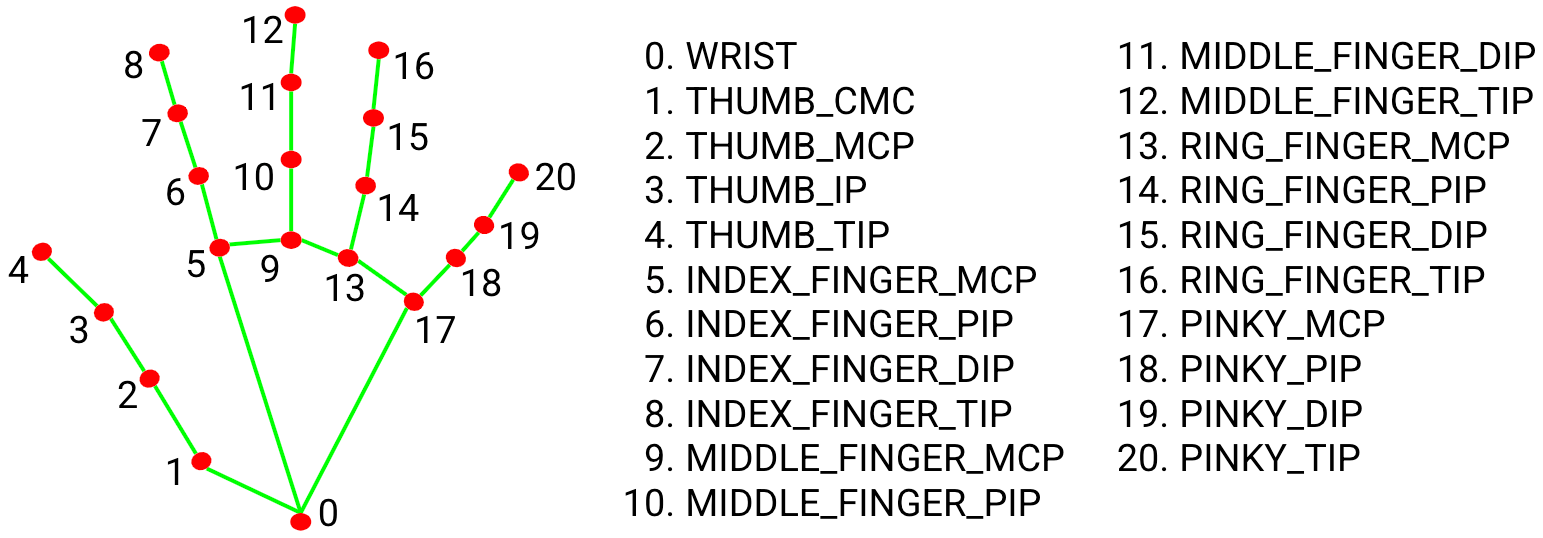
\includegraphics[width=15cm]{../images/hand_landmarks.png}
        \caption{Elementy charakterystyczne dłoni}
    \end{center}
\end{figure}

\quad Pierwszym elementem określanym przez enumerator jest nadgarstek. Dalej znajduje się reszta indeksów, oznaczająca resztę części palców i dłoni.  

\begin{lstlisting}[caption={Przykładowe wykorzystanie \textbf{mp\_hands}},captionpos=b,language=python]
    x = hand.landmark[self.mp_hands.HandLandmark.WRIST].x
\end{lstlisting}

\quad Tak jak zostało to ukazane powyżej, enumerator może zostać wykorzystany, na przykłd do odczytu wpółrzędnej danego puntku. Jest to ułatwienie, dzięki któremu program staje się czytelnieszy dla programisty lub osoby przeglądającej program. 

\subsection{Struktura results}

\quad Struktura \textbf{results} jest obiektem, który przechowuje informacje zwrócone przez metodę \textbf{hands.process()}. Klasa OpenLeap korzysta z dwóch typów informacji zwracanych przez tą metodę. 

\begin{itemize}
    \item \textbf{multi\_hand\_landmarks} - obiekt przechowujący dane o pozycjach wszystkich elementów dłoni. Przykład wykorzystania został przedstawiony powyżej. 
    
    \begin{lstlisting}[caption={Przykład elementu obiektu},captionpos=b,language=python]
        [landmark {
            x: 0.7409825921058655
            y: 0.6843034029006958
            z: 0.0
            }
            .s
            .
            .
            landmark {
            x: 0.7874422073364258
            y: 0.26234549283981323
            z: -0.16528795659542084
            }
        ]
    \end{lstlisting}
    

    \item \textbf{multi\_handedness} - lista przechowująca dane o wszysktich dłoniach widocznych na obraze. Danymi są indeks, typ dłoni oraz punktacja określającą pewność poprawnego rozpoznania dłoni. 
    \begin{lstlisting}[caption={Przykład elementu obiektu},captionpos=b,language=python]
        [classification {
                index: 1
                score: 0.9482673406600952
                label: "Right"
            }
        ]
    \end{lstlisting}
\end{itemize}

\subsection{Dataclass}

\quad Strukura typu \textbf{Dataclass} pozwala na stworznie struktury podobnej do \textbf{struct} istniejącej w języku programowania \textbf{C}. Taka klasa pozwala na storzenie obiektu składającego się jedynie z atrybutów wymaganych do opisue elementów klasy kontrolera. Dodatkowym atutem takiej klasy jest możliwość prostego odczytu zapisanych danych, korzystając z operatora kropki, a nie z operatrów opisujących słownik lub listę. 

\begin{lstlisting}[language=python]
    @dataclass
    class Data:
        x : float = 0
        y : float = 0
        z : float = 0
        distance: float = 0.0
        angle: float = 0.0
        gesture: str = None
\end{lstlisting}

\quad W języku Python stworzenie klasy typu \textbf{dataclass} zaczyna się od zapisania dekoratora. W tym wypadku nie jest wymagana funkcja inicjalizująca obiekt, czyli \textbf{\_\_init\_\_}. Parametetry początkowe można podać w chwili tworzenia obiektu, lub później. W programie zostały przypisane wartości początkowej, tak jak w przykładzie powyżej. 

\subsection{Słownik}

\quad Instancja stworzonego typu \textbf{Data} zostnie zainicjowana dla każdej dłoni (lewej oraz prawej). Te instacje zostaną zapisane w słowniku. 

\begin{lstlisting}[language=python]
    data = {'right':Data(), 'left':Data()}
\end{lstlisting}

\quad Taka konstrukcja pozwoli użytkownikowi w prosty i przejrzysty sposób na odnajodowania potrzebnych wartości oraz informacji. 

\subsection{Pickle}
\quad Modele matematyczne, które zostaną wytrenowane muszą zostać zapisane, tak aby można było je wykorzystać ponownie. Z tego powodu został wykorzystany plik typi \textbf{pickle}, który umożliwia zapis zmiennych oraz obiektów w postaci binarnej. Dzięki czemu można je wykorzystać ponownie pomimo restartu programu. 

\section{Rozpoznawanie dłoni}

\quad Pierwszym elementem projektu jest rozpoznanie dłoni poprzez wyznacznie pozycji elementów charakterystycznych. Pozycja każdego z tych elementów, jak już zostało to opisane, jest względna według lewego górnego rogu obrazu kamery. 

\begin{figure}[H]
    \begin{center}
        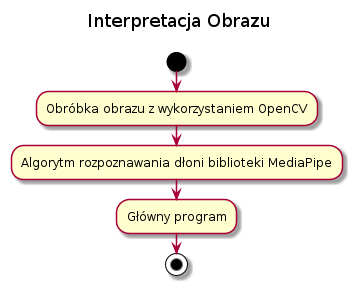
\includegraphics[width=10cm]{../images/image_processing.png}
        \caption{Przygotowanie obrazu}
    \end{center}
\end{figure}

\quad W pierwszym kroku obraz powinnien zostać pozyskany z kamery oraz odpowiednio przetworzony przez funkcje biblioteki OpenCV. 

\quad Kolejnym krokiem jest rozpoznanie elementów charakterystycznych dłoni przez model biblioteki MediaPipe. 

\quad Na końcu powinna zostać wykonana główna część programu. Na przykład ropoznanie gestu czy obliczenia kąt obrotu. 

%%%%%%%%%%%%%%%%%%%%%%%%%%%%%%%%%%%%%%%%%%%%%%%%%%%%%%%%%%%%%%%%%%%%
%%%%%%%%%%%%%%%%%%%%%%%%%%%%%% OPEN CV %%%%%%%%%%%%%%%%%%%%%%%%%%%%%
%%%%%%%%%%%%%%%%%%%%%%%%%%%%%%%%%%%%%%%%%%%%%%%%%%%%%%%%%%%%%%%%%%%%
\subsection{OpenCV - przygotowanie obrazu z kamery}

\quad W pierszym kroku należy zainicjalizować obiekt obsługujący kamerę. Argumntem jest identyfikator określający, która kamera podłączona do systemu ma zostać wykorzystana. W przypadku kiedy dostępna jest tylko jedna kamera wystarczy wpisać wartość równą 0, tak jak poniżej.  

% \inputminted[firstline=51, lastline=52]{python}{../OpenLeap.py}

\lstinputlisting[language=python, firstline=81, lastline=81]{../openleap/openleap/OpenLeap.py}

\quad W metodzie \textbf{main()} w pierwszym kroku warunek określa czy zostało otwarte połączenia z kamerą. Jeśli tak to należy pobrać z niej aktualną klatkę obrazu (\textbf{frame}). 

\lstinputlisting[language=python, firstline=293, lastline=301]{../openleap/openleap/OpenLeap.py}

\quad Model rozpoznający dłoń korzysta z przestrzeni barw RGB (red, green, blue), a nie BGR (blue, green, red). Dlatego należy obraz przekształcić właśnie na przesrzeń RGB. Dodatkowo, obraz powinnien zostać obrócony horyzntalnie, tak aby stworzył lustrzane odbicie względem użytkownika ustawionego na przeciwko kamery. 

\lstinputlisting[language=python, firstline=302, lastline=307]{../openleap/openleap/OpenLeap.py}

\quad Flage \textbf{writeable} ustawiona na \textbf{False} pozwala na uzyskanie lepszej wydajności przy przetwarzaniu obrazu w ramach modelu rozpoznającego dłonie. 

\lstinputlisting[language=python, firstline=308, lastline=316]{../openleap/openleap/OpenLeap.py}

\quad Przestrzeń barw zostaje przywrócona do RGB, aby była mogła zostać poprawnie wyświetlona przez funkcję biblioteki OpenCV. 

\lstinputlisting[language=python, firstline=318, lastline=320]{../openleap/openleap/OpenLeap.py}

% \inputminted[language=python, firstline=272, lastline=297]{python}{../openleap/openleap/OpenLeap}

%%%%%%%%%%%%%%%%%%%%%%%%%%%%%%%%%%%%%%%%%%%%%%%%%%%%%%%%%%%%%%%%%%%%
%%%%%%%%%%%%%%%%%%%%%%%%%%%% MEDIA PIPE %%%%%%%%%%%%%%%%%%%%%%%%%%%%
%%%%%%%%%%%%%%%%%%%%%%%%%%%%%%%%%%%%%%%%%%%%%%%%%%%%%%%%%%%%%%%%%%%%

\subsection{MediaPipe - Elementy charakterystyczne}

\quad Pozycje nadgarstka, paliczków oraz stawów dłoni zostaną wykorzystane do obliczenia obrotu dłoni względem punkut 0 oraz do wytrenowania modeli uczenia maszynowego, których zadaniem będzie rozpoznawnie wybranych gestów. 

\subsection{Generowanie grafiki dłoni}

\quad Generowanie grafiki nałożonej na daną dłoń wykonuje się przy pomocy przygotowanej funkcji biblioteki MediaPipe, która współpracuje z OpenCV.   

\section{Pomiary oraz inne ważne elementy}

\subsection{Pozycja dłoni}

\subsection{Obrót dłoni}

\subsection{Odległość między palcami}

%%%%%%%%%%%%%%%%%%%%%%%%%%%%%%%%%%%%%%%%%%%%%%%%%%%%%%%%%%%%%%%%%%%%
%%%%%%%%%%%%%%%%%%%%%%%%%%% SciKit Learn %%%%%%%%%%%%%%%%%%%%%%%%%%%
%%%%%%%%%%%%%%%%%%%%%%%%%%%%%%%%%%%%%%%%%%%%%%%%%%%%%%%%%%%%%%%%%%%%


% \section{Uczenie Maszynowe}

\section{Rozpoznawanie gestów}

\subsection{Przygotowanie modeli uczenia maszynowego}
\quad Celem programu będzie stworzenie modeli matematycznych przy pomocy metod uczenia maszynowego, których celem będzie rozpoznawanie gestów dłoni. Proces tworzenie takiego modelu można podzielić na trzy kroki przedstawione na schemacie 6.3. 

\begin{figure}[H]
    \begin{center}
        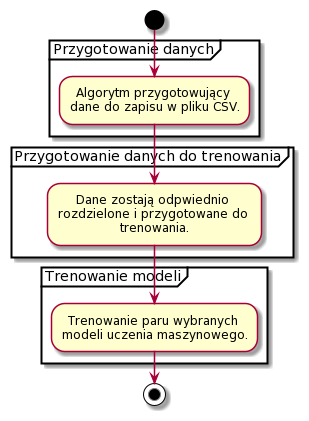
\includegraphics[width=8cm]{../images/full_algorithm.png}
        \caption{Ogólny algorytm przygotowania modeli uczenia maszynowego}
    \end{center}
\end{figure}

\quad Całość programu została napisana w notatniku Jupyter. Pozwala to na wykonanie pewnych części programu osobno, niezależnie od reszty programu. W praktyce każdy blok opisany w powyższym schemacie UML ma swoje odwzorowanie w notatniku. Na przykład, część zapisująca współrzędne do pliku będzie wykonywana tyle razy ile jest gestów do wytrenowania. 

\subsection{Zebranie danych}
\quad Algorytm zebrania danych polega na pobraniu współrzędnych oszacowanych przez model MediaPipe. Należy pamiętać o tym, że środek układu współrzędnych znajduje się lewym górnym rogu obrazu kamery. Oznacza to, że współrzędne w tej postaci nie nadają się do wyuczenia modelu matematycznego. Gest nie powinnien być rozpoznawany na podstawie pozycji dłoni w obrazie lub jej odległości od kamery. Należy się tych zależności pozbyć. 

\begin{figure}[H]
    \begin{center}
        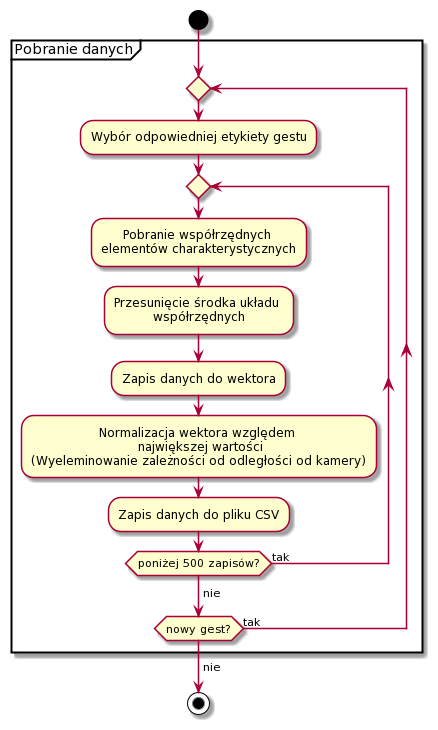
\includegraphics[width=10cm]{../images/get_data.png}
        \caption{Ogólny algorytm przygotowania modeli uczenia maszynowego}
    \end{center}
\end{figure}

\quad Gest dłoni, można scharakteryzować na podstawie pozycji elementów dłoni. Podstawowym problemem jest fakt, że pozycje elementów charakterystycznych są opisane względem układu współrzędnych, którego środek znajduje się w lewym górnym rogu obrazu pobranego z kamery. Pozycja dłoni na obrazie nie ma żadnego znaczenia w kwestii określania gestu. Poprawnie przygotowane pozycje elementów powinnny zostać pozbawione zależności od pozycji dłoni względem obrazu. 
\quad Przygotowanie danych do przetworzenia będzie wymagało paru opercaji matematycznych. W takim wypadku należy przprowadzić transformację, tutaj akurat przesunięcie układu współrzędnych do pozycji nadgarstka. Taka operacja pozwoli na opis pozycji elementów względem nagarstka. Ostatecznie pozbywamy się pozycji nadarstka z wektora danych, ponieważ jest ona środkiem nowego układu współrzędnych. 

\quad \textbf{Macierz przesunięcia}

\begin{equation*}
    M_p = 
    \begin{bmatrix}
    1 & 0 & 0 & -x_0 \\
    0 & 1 & 0 & -y_0 \\
    0 & 0 & 1 & -z_0 \\
    0 & 0 & 0 & 1
    \end{bmatrix}
\end{equation*}

\quad Tak naprawdę, przesunięcie układu współrzędnych w osi Z nie będzie miało miejsca. Wartości współrzędnej Z reszty elementów, oprócz elementu z indeksem równym 0, czyli nadgarstka, są określane właśnie nadgarstka. Dlatego też, macierz przesunięcia w osi Z jest równa 0. 

\begin{equation*}
    M_p = 
    \begin{bmatrix}
    1 & 0 & 0 & -x_0 \\
    0 & 1 & 0 & -y_0 \\
    0 & 0 & 1 & 0 \\
    0 & 0 & 0 & 1
    \end{bmatrix}
\end{equation*}

\quad Aby dane mogły zostać zinterpretowane przez algorytmy ucznenia maszynowego muszą one zostać przedstawione w postaci jednowymiarowej. Aktualna postać macierzy przedstawiającej wpółrzędne elementów charakterystycznych ma następującą postać. Indeksy współrzędnych są równoznaczne z indeksami elementów dłoni. 

\begin{equation*}
    M_p = 
    \begin{bmatrix}
    x_1' & y_1' & z_1' \\
    x_2' & y_2' & z_2' \\
        & \vdots &     \\
    x_{21}' & y_{21}' & z_{21}'
    \end{bmatrix}
\end{equation*}

Dane w postaci jednowymiarowej mają postać następującego wektora. 

\begin{equation*}
    A_f=
    \begin{bmatrix}
        x_1 & y_1 & z_1 & x_2 & y_2 & \cdots & y_{21} & z_{21}
    \end{bmatrix}
\end{equation*}


\quad Drugim krokiem jest uniezależnienie pozycji elementów od odległości dłoni od kamery. Najprostszym rozwiązaniem jest normalizacja wektora danych względem największej bezwzględnej wartości. 

\quad \textbf{Normalizacja}

% \begin{equation*}
%     A_n=
    % \begin{bmatrix}
    %     x_1 & y_1 & z_1 & x_2 & y_2 & \cdots & y_{21} & z_{21}
    % \end{bmatrix}
% \end{equation*}


\begin{equation*}
    A_n=\dfrac{A_f}{max(abs(A_f))}
\end{equation*}

\quad Każdy nowy wektor zostaje zapisany do pliku CSV z odpwowiednią etykietą. Zebrane dane posłużą do wytrenowania algorytmów uczenia maszynowego.     

\subsection{Budowa pliku CSV}
\quad Dane zapisane w pliku CSV opisują przykładowe współrzędne wszysktich elementów dłoni wraz z przypisaną etykietą oznaczającą gest. 

\subsection{Metody klasyfikacji - uczenie maszynowe}

\quad Przygotowane dane zostają odczytane z pliku CSV. W pierwszym kroku należy rozdzielić je na dwie części: współrzędne (dane wejściowe) oraz etykiety (dane wyjściowe). W kolejnym kroku należy te dwie grupy podzielić na grupę trenującą i grupę testową. Zadaniem grupy testowej będzie trenowanie wybranych modeli matematycznych, a grupy testowej przetestowanie ich dokładności. 

\begin{figure}[H]
    \begin{center}
        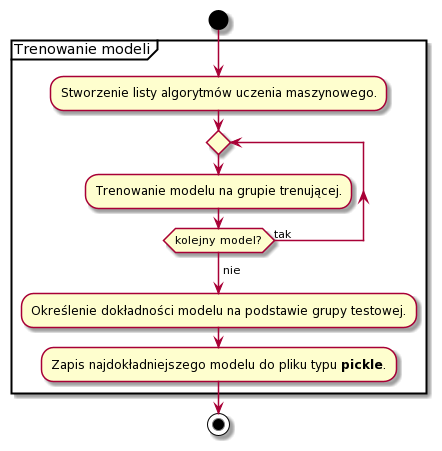
\includegraphics[width=11cm]{../images/train_models.png}
        \caption{Ogólny algorytm przygotowania modeli uczenia maszynowego}
    \end{center}
\end{figure}

\quad W celu wybrania najlepszej metody klasyfikacji, zostnie wybranych kilka algorytmów. Każdy z nich stworzy swój model, a ostatecznie zostanie sprawdzona ich poprawności z wykorzystaniem grupy testowej. Model z najepszym wynikiem zostanie zapisany do pliku typu \textbf{pickle}. W języku Python pliki typu \textbf{pickle} pozwalają na zapis zmiennych, obiektów lub innych struktur danych, które mają zostać wykorzystane w po zakończeniu programu. 

\subsection{Wybrane algorytmy klasyfikujące}

\quad Do wytrenowania modeli uczenia maszynowego z biblioteki SciKit Learn zostały wybrane następujące algorytmy. 

\begin{itemize}
    \item Logistic Regression
    \item Nearest Centroid 
    \item Decision Tree Classifier 
    \item Random Forest Classifier 
    \item SGD Classifier
    \item Gradient Boosting Classifier
    \item MPL Classifier
\end{itemize}

\subsection{Badanie dokładności każdego z algorytmów}

\subsection{Ponowne wykorzystanie modelu}

\quad Gotowy model pobieramy i testujemy w przykładowym programie. 

\section{Paczka PyPi}

\subsection{Budowa paczki}

\quad Ostatecznym krokiem jest przygotowanie programu w formie paczki, która zostanie udostępniona na platformie PyPi. Wygama to przygotowania odpowiednich plików konfiguracyjnych oraz zostosowania stosownych narzędzi do stworznie pliku \textbf{wheel} oraz \textbf{tar}. 

\subsection{Struktura Paczki}
\quad Pierwszm krokiem jest przygotowanie odpowiedniej struktury paczki. Do tego celu został stworzony folder o poniższej strukturze. W tym folderze znajdują się wszystkie potrzebne elementy paczki. W podfolderze o tej samej nazwie znajduje się główna części modułu, czyli plik .py, w którym zapisana jest klasa OpenLeap. Dodatkowo w tym folderze znajdują się pliki typu \textbf{pickle}, w których zapisane są modele rozpoznające gesty.

\begin{figure}
\centering
    \begin{minipage}{7cm}
        \dirtree{%
        .1 openleap.
        .2 openleap.
        .3 \hyperref[openleap-file1]{\_\_init\_\_.py}.
        .3 \hyperref[openleap-file2]{OpenLeap.py}.
        .3 \hyperref[openleap-file3]{gesture\_recognition.pkl}.
        .3 \hyperref[openleap-file4]{sign\_language\_alphabet.pkl}.
        .2 LICENSE.
        .2 MANIFEST.
        .2 README.md.
        .2 setup.py.
        } 
    \end{minipage}
    \caption{Struktura paczki PyPi}
\end{figure}

\subsection{Pliki Konfiguracyjne}
\quad Pliki setup.py oraz MANIFEST są plikami, które odpowiadają za konfigurację oraz opis paczki. W pliku setup.py zapisany jest numer aktualnej wersji, autor, kontakt do autora, nazwa paczki itp. 

\quad 


% \subsection{Plik setup.py}
\subsection{Załadowanie paczki do repozytorium}

\quad Przed załadowaniem paczki do repozytorium, należy stworzyć zapakowaną paczkę źródłową, na przykład typu .tar oraz plik typu WHEEL. Oba pliki spełniają tą samą funkcję, czyli przechowywnie niezbędnych elementów paczki oraz umożliwiają ich instalację na systemie użytkownika. Plik WHEEL pozwala na dużo szybszy proces instalacji niż instalacja ze źródła, czyli paczki typu .tar. 
